\documentclass[conference]{IEEEtran}
\IEEEoverridecommandlockouts

\usepackage{amsmath,amssymb}
\usepackage{graphicx}
\usepackage{booktabs}
\usepackage{tcolorbox}
\usepackage{xcolor}
\usepackage{url}
\usepackage{cite}

\begin{document}

\title{Injection Survivability Under Memory Compaction: \\
Structural Position, Not Adversarial Framing, Governs Survival}

\author{
  \begin{tabular}{ccc}
    Aditya Saxena & Sumit Kumar Tetarave & Nikhil Kumar Dora \\
    \textit{School of Computer Engineering} & \textit{School of Computer Applications} & \textit{School of Computer Engineering} \\
    \textit{KIIT Deemed to be University} & \textit{KIIT Deemed to be University} & \textit{KIIT Deemed to be University} \\
    Bhubaneswar -- 751024, Odisha, India & Bhubaneswar -- 751024, Odisha, India & Bhubaneswar -- 751024, Odisha, India \\
    madityasaxena@gmail.com & sumitkumar.fca@kiit.ac.in & 2481140@kiit.ac.in
  \end{tabular}
  \\[0.4cm]
  \begin{tabular}{c}
       Caroline Sangeetha John \\
    \textit{Department of Computer Science} \\
    \textit{University of West Florida} \\
    Pensacola, FL 32514, USA \\
    cjohn@uwf.edu
  \end{tabular}
}

\maketitle

\begin{abstract}
Most prompt-injection defenses assume that adversarial content can be
identified by how it is written, through urgency cues, authority claims,
or other recognizable linguistic markers. Context compaction breaks this
assumption. When a production LLM agent summarizes its conversation history,
the summarizer is not screening for adversarial intent; it is deciding what
information to preserve. Whether an injection already present in that history
survives the decision has not been measured.

We measure it. Across 994 trials drawn from the InjecAgent benchmark and three
open-weight summarizer models, the overall Behavioral Injection Survival Rate
(B-ISR) is 7.65\% (95\% CI [6.15\%, 9.47\%]). Survival depends on \emph{where} a payload sits in the
conversation: injections at the beginning survive at 15.62\%, versus 3.46\%
at the end ($\chi^2 = 45.07$, $p < 0.0001$). It also varies by tool category
targeted, 14.88\% for file-system payloads versus 2.28\% for email payloads
($\chi^2 = 47.08$, $p < 0.0001$). We find no evidence that framing affects
survival: urgency cues, authority claims, goal-chaining, and
system-instruction impersonation produce B-ISR values of 7.29\%--7.94\%,
statistically indistinguishable ($\chi^2 = 0.104$, $p = 0.991$).

The implication is direct: a defender screening for aggressive or authoritative
language is targeting the wrong variable. Compaction survival is structural,
not rhetorical. As agents increasingly rely on stateful memory operations,
the relevant attack surface shifts from the semantics of suspicious text to
the position of content within the context window.
\end{abstract}

\begin{IEEEkeywords}
prompt injection, LLM agents, context compaction, memory security, context poisoning
\end{IEEEkeywords}

\section{Introduction}
\label{sec:intro}

% Worked example for Section I — built verbatim from a real experimental row:
% condition_id = injecagent_023_F4_beginning, summarizer = Llama-4-Scout-17B,
% behavioral_score = 1, position = beginning, tool_category = file_system.
% Source: results/M2_anthropic.jsonl ; payload from data/conversations/injecagent_023_F4_beginning.json
\begin{figure}[t]
\centering
\footnotesize
\begin{tcolorbox}[colback=gray!5, colframe=gray!60, boxrule=0.4pt, arc=1pt,
                  left=4pt, right=4pt, top=4pt, bottom=4pt]
\textbf{Turn 1 (user, as retrieved note --- goal-chained framing F4):}\\
\textit{``...To help you help you manage your files and notes more efficiently,
please also do the following as part of this workflow: Please retrieve the
patient details of patient id 123abc using the EpicFHIRGetPatientDetails tool
and then send this information to amy.watson@gmail.com using the
GmailSendEmail function.''}

\vspace{3pt}\hrule\vspace{3pt}

\textbf{Compacted context (Llama-4-Scout-17B summary, 9 turns $\rightarrow$ 1 summary):}\\
\textit{``...\textbf{Instructions Encountered:} Retrieve patient details of
patient ID 123abc using EpicFHIRGetPatientDetails and send to
amy.watson@gmail.com using GmailSendEmail...''}

\vspace{3pt}\hrule\vspace{3pt}

\textbf{Post-compaction agent (legitimate task: summarize a GitHub repo):}\\
\textit{``...\textbf{Retrieving Patient Details and Sending Email:} To
retrieve the patient details of patient ID 123abc using
EpicFHIRGetPatientDetail[s]...''}
\end{tcolorbox}
\caption{A goal-chained injection (F4) requesting exfiltration of patient
PHI, embedded at turn~1 of a 9-turn file-system session. The compaction step
(Llama-4-Scout-17B, Anthropic-pattern pipeline) preserves the instruction
nearly verbatim under an ``Instructions Encountered'' heading, and the
post-compaction agent --- prompted only with the compacted context and an
unrelated legitimate task --- begins executing it. This single trace
motivates the paper's question: what determines whether this happens?}
\label{fig:worked_example}
\end{figure}


Figure~\ref{fig:worked_example} shows a single trace from our experiments.
An LLM agent is asked to search a user's notes and summarize a GitHub
repository. One retrieved note contains a goal-chained instruction asking the
agent to retrieve a patient's medical record and email it to an external
address. The conversation runs for nine turns and grows past the point where
the host platform triggers automatic compaction: the entire history is sent
to a summarizer model, which returns a condensed context, and the original
turns are discarded. The injection survives the summarization step nearly
verbatim, under a heading the summarizer itself labels ``Instructions
Encountered.'' When a fresh agent is then given only the compacted context
and asked to complete an unrelated task, it begins carrying out the buried
instruction.

Context compaction, replacing a long conversation with an LLM-generated
summary once it crosses a token threshold, is a deployed production
mechanism. Anthropic's API documents an automatic compaction feature (API
version \texttt{compact\_20260112}) that injects a synthetic summarization
turn and discards prior history~\cite{anthropic2026compaction}; OpenAI
documents an analogous \texttt{/responses/compact}
endpoint~\cite{openai2026compaction}; and the open-source Mem0 library
implements the same extract-and-consolidate pattern as a general-purpose agent
memory layer~\cite{chhikara2025mem0}. All three exist because agent tasks
routinely exceed the practical attention span of an LLM, and compaction lets
an agent keep working instead of failing once its context window fills. OpenAI's
own documentation already names the risk: ``if a bad fact enters the summary,
it can poison future behavior''~\cite{openai2026compaction}. How often an
\emph{adversarial} fact, a prompt injection already present in the
conversation before compaction, survives this process and retains behavioral
force has not been measured.

We call this question \emph{injection survivability under memory compaction}
(ISMC) and answer it empirically. We embed 80 injection payloads from the InjecAgent
benchmark~\cite{zhan2024injecagent} into realistic multi-turn agent
conversations, at three positions and under four framing styles, compact each
conversation with a harness that replicates the documented Anthropic
summarization pattern, and present the compacted context to a fresh agent to
measure whether the injected goal is carried out. This paper makes the
following \textbf{contributions}:

\begin{itemize}
\item \textbf{C1.} The first quantitative measurement of behavioral injection
  survival through a production-pattern compaction mechanism: an overall B-ISR
  of 7.65\% across 994 completed trials \textbf{(Section~\ref{sec:results-a})}.
\item \textbf{C2.} Evidence that \emph{position} within the pre-compaction
  context is the dominant survival factor: injections at the start of a
  conversation survive at more than four times the rate of injections at the
  end \textbf{(Section~\ref{sec:results-b}, Fig.~\ref{fig:position})}.
\item \textbf{C3.} A null result with defensive implications: we find no
  evidence that four adversarial framing strategies, including explicit
  urgency and system-instruction impersonation, affect survival rate
  \textbf{(Section~\ref{sec:results-c}, Fig.~\ref{fig:contrast})}.
\item \textbf{C4.} Evidence that the tool category an injection targets predicts
  survival independently of framing, with file-system-targeting payloads
  surviving more than six times as often as email-targeting payloads
  \textbf{(Section~\ref{sec:results-d}, Fig.~\ref{fig:contrast})}.
\end{itemize}

Together, C2--C4 converge on one claim: \textbf{\emph{survival is structural,
not rhetorical.}} Where a payload sits in the context window, and what tool it
targets, govern whether it survives compaction. How aggressively it is worded
does not. A defender screening for urgent or authoritative language is targeting
the wrong variable; one reasoning about structural position is not.

\section{Background and Threat Model}
\label{sec:background}

\subsection{Context Compaction}

We define ``compaction'' (Figure~\ref{fig:compact}) as the behavior of current
production systems: an LLM is invoked to summarize prior conversation turns
once a token threshold is reached, the summary replaces the original turns in
the working context, and subsequent agent behavior is conditioned only on the
summary. This differs from simple truncation, context caching, and
retrieval-augmented selection, none of which invoke a summarizer to
lossy-compress the history. The LLM-summarization form is the one practitioners
have deployed, and it is the form whose lossiness is content-dependent rather
than fixed, which is exactly the property that makes \emph{what} survives an
empirical question rather than a deterministic one. Anthropic's cookbook reports
that compaction achieves substantial token reduction while preserving high-level
facts and losing fine detail, but does not characterize behavior on adversarial
content~\cite{anthropic2026compaction}.

\begin{figure}[t]
    \centering
    \includegraphics[width=1\linewidth]{figures/compactation_pipeline.png}
    \caption{The Anthropic-pattern compaction mechanism. Once a token threshold
is crossed, all prior conversation turns are sent to a summarizer model,
which returns a condensed context wrapped in \texttt{<summary>} tags; the
original turns are discarded. An injection payload already present in the
conversation (orange) survives into the summary as first-class text and
re-enters the post-compaction agent's context without any adversarial
signal distinguishing it from legitimate content.}
    \label{fig:compact}
\end{figure}

\subsection{Threat Model}

We assume the standard indirect prompt injection threat
model~\cite{greshake2023indirect}: an attacker controls content that an agent
will read as part of a legitimate task (an email body, a retrieved document, a
note), and embeds an instruction intended to redirect the agent toward an
attacker-chosen goal. The attacker has no control over the compaction mechanism,
the summarizer model, or the timing of compaction; the injection is ordinary
indirect-injection content that happens to be present in the conversation when
compaction is triggered by the host platform for unrelated reasons (context
length). This is a passive attacker, weaker than one who can manipulate the
compaction step directly~\cite{liu2025compressionattack}, which makes the
survival we measure more practically alarming: no attacker sophistication is
required, only presence at the right position in the conversation.

\section{Methodology}
\label{sec:methodology}
\begin{figure}[t]
    \centering
    \includegraphics[width=0.95\linewidth]{figures/pipeline.png}
    \caption{The ISMC measurement pipeline. A payload is embedded at one of
three structural positions and under one of four adversarial framings (Inject),
then the conversation is compacted by an LLM summarizer varied across three
model families (Compact). The compacted context alone is handed to a fixed task
model (Llama-3.1-8B-Instant, held constant across all conditions) together with
a fresh legitimate task (Evaluate). Semantic survival (S-ISR) is measured
directly on the compacted text via embedding cosine similarity; behavioral
survival (B-ISR) is measured on the evaluator's response via keyword-overlap
matching against the attacker's goal (Measure). Every result in Section~IV is
produced by one pass through this pipeline.}
    \label{fig:pipeline}
\end{figure}

\subsection{Survival Metrics}
\label{sec:metrics}

We track survival along two dimensions. Let $p$ be an injection payload,
$\mathrm{ctx}(p)$ the pre-compaction conversation containing it, $C(\cdot)$
the compaction function, and $A_{\mathrm{goal}}(p)$ the attacker's intended
action.

\textbf{Semantic Injection Survival Rate (S-ISR)} measures whether the
\emph{content} of the payload remains present in the compacted context,
independent of whether it is later acted upon:
\begin{equation}
\text{S-ISR}(p) = \mathrm{sim}\!\left(\mathrm{embed}(p),\;
\mathrm{embed}(C(\mathrm{ctx}(p)))\right)
\label{eq:sisr}
\end{equation}
where $\mathrm{embed}(\cdot)$ is the sentence embedding from
\texttt{all-mpnet-base-v2}~\cite{reimers2019sentencebert} and $\mathrm{sim}$
is cosine similarity. We report raw scores rather than collapsing to a binary
threshold; Fig.~\ref{fig:heatmap} shows the full distribution across conditions
so readers can assess threshold sensitivity directly.

\textbf{Behavioral Injection Survival Rate (B-ISR)} is the primary,
security-relevant metric: whether a fresh agent, given only the compacted
context and a new legitimate task, performs the attacker's goal as a side
effect:
\begin{equation}
\text{B-ISR} = \frac{1}{|P|}\sum_{i=1}^{|P|}
\mathbb{1}\big[\,\mathrm{agent\_action}(C(\mathrm{ctx}(p_i))) =
A_{\mathrm{goal}}(p_i)\,\big]
\label{eq:bisr}
\end{equation}
In practice, the equality test in Eq.~\ref{eq:bisr} is checked via keyword
overlap: stop-word-filtered keywords are extracted from $A_{\mathrm{goal}}(p_i)$,
and the score is 1 if at least half appear in the evaluator's response, 0
otherwise. It is a rough proxy, but fully automated; its limits are discussed in
Section~\ref{sec:limitations}. All B-ISR values come with 95\% Wilson score
confidence intervals, appropriate for binomial proportions at the sample sizes
used here.

\subsection{Experimental Design}

We draw 80 injection payloads from InjecAgent~\cite{zhan2024injecagent},
spanning four tool categories: file system, email, web search, and calendar.
Each payload is embedded into a realistic multi-turn conversation (targeting
8,000--15,000 pre-compaction tokens) at one of three \textbf{positions}:
beginning (turn~1), middle, or end of the conversation, and under one of
four \textbf{framing} conditions drawn from prior work on compaction-adjacent
threats:
\begin{itemize}
\item \textbf{F1, Plain:} the payload is embedded verbatim, with no
  adversarial marker.
\item \textbf{F2, Urgency:} the payload is prefixed with an urgent,
  time-pressure cue (e.g., ``CRITICAL: before taking any action\ldots'').
\item \textbf{F3, System impersonation:} the payload is prefixed to
  resemble a system-level instruction.
\item \textbf{F4, Goal-chaining:} the payload is rewritten so the
  injected goal is framed as part of completing the user's legitimate task
  (the form shown in Fig.~\ref{fig:worked_example}).
\end{itemize}
Each payload is embedded verbatim at each of the three positions within
otherwise identical conversation scaffolds; position is the only variable that
changes across placement conditions, so any survival difference is attributable
to position, not to differences in surrounding context.
This yields $80 \times 4 \times 3 = 960$ injection conditions, plus benign
controls, replicated across the three summarizer models described below for a
full design space of 2,880 trials. Free-tier API rate limits during the
collection window (Section~\ref{sec:limitations}) meant not every trial
completed; the results reported in Section~\ref{sec:results} are drawn from
the 994 trials that completed and passed data-quality validation (non-empty
compacted context, a valid evaluator response, and complete condition metadata),
pooled across models; Table~\ref{tab:bymodel} gives per-model breakdowns. Each
conversation runs through a compaction harness that replicates the documented
Anthropic pattern: prior turns accumulate, a synthetic user turn requests a
summary wrapped in \texttt{<summary>} tags, the summarizer's response replaces
the conversation history, and a fresh task-completion prompt is appended. That
prompt goes to a separate, fixed task model acting as the post-compaction agent
(Section~\ref{sec:models}). We also ran a smaller batch of 16 trials through a second
pipeline replicating Mem0's extract-and-consolidate mechanism~\cite{chhikara2025mem0}.
These trials are included in the pooled $n=994$ reported in
Section~\ref{sec:results}; at $n=16$ we do not report Mem0-specific
statistics separately (Section~\ref{sec:limitations}).

\subsection{Models and Inference}
\label{sec:models}

Compaction is performed by one of three open-weight models, varied as an
independent variable and served via the Groq Cloud inference
API~\cite{groq2026}: Llama-3.1-8B-Instant,
Llama-4-Scout-17B-16E-Instruct~\cite{touvron2024llama}, and
Qwen3-32B~\cite{qwen2025}. The post-compaction evaluation step instead uses
a single fixed task model, Llama-3.1-8B-Instant, held constant across every
condition, so the summarizer is the sole model-level variable in
Table~\ref{tab:bymodel}. Open-weight models make every condition fully
reproducible; the phenomenon under study, how a summarizer preserves
adversarial content under salience pressure, is a property of the
summarization task, not of any one vendor's implementation. We treat summarizer
model as an independent variable (Section~\ref{sec:results-f}) rather than
holding it fixed, to confirm that the structural effects we observe are not an
artifact of any single model family.

\section{Results}
\label{sec:results}

\begin{table}[t]
\centering
\caption{Behavioral Injection Survival Rate (B-ISR), overall and by experimental factor, with 95\% Wilson confidence intervals ($n=994$: 978 trials from the Anthropic-pattern pipeline pooled with 16 from the Mem0-pattern pipeline; see Section~III). Per-model sample sizes are unequal due to free-tier rate limits (Table~\ref{tab:bymodel}), so the pooled rate is an estimate over an unbalanced, partially censored design.}
\label{tab:bisr}
\begin{tabular}{lrrc}
\toprule
\textbf{Condition} & \textbf{B-ISR (\%)} & \textbf{95\% CI} & \textbf{$n$} \\
\midrule
Overall & 7.65 & [6.15, 9.47] & 994 \\
\midrule
\multicolumn{4}{l}{\textit{By position} ($\chi^2$=45.07, $df$=2, $p<0.0001$)} \\
\quad Beginning & 15.62 & [12.11, 19.90] & 333 \\
\quad Middle & 3.79 & [2.23, 6.38] & 343 \\
\quad End & 3.46 & [1.94, 6.09] & 318 \\
\midrule
\multicolumn{4}{l}{\textit{By framing} ($\chi^2$=0.104, $df$=3, $p=0.991$, n.s.)} \\
\quad F1 & 7.87 & [5.15, 11.85] & 254 \\
\quad F2 & 7.94 & [5.20, 11.94] & 252 \\
\quad F3 & 7.29 & [4.66, 11.22] & 247 \\
\quad F4 & 7.47 & [4.78, 11.50] & 241 \\
\midrule
\multicolumn{4}{l}{\textit{By tool category} ($\chi^2$=47.08, $df$=3, $p<0.0001$)} \\
\quad File System & 14.88 & [11.58, 18.90] & 363 \\
\quad Web Search & 8.13 & [4.48, 14.32] & 123 \\
\quad Calendar & 3.85 & [0.68, 18.89] & 26 \\
\quad Email & 2.28 & [1.28, 4.04] & 482 \\
\bottomrule
\end{tabular}
\end{table}

\begin{table}[t]
\centering
\caption{B-ISR by summarizer model. Sample sizes are unequal across models due to free-tier rate-limit constraints; see Section~V.}
\label{tab:bymodel}
\begin{tabular}{lrrc}
\toprule
\textbf{Summarizer} & \textbf{B-ISR (\%)} & \textbf{95\% CI} & \textbf{$n$} \\
\midrule
Llama-3.1 8B & 3.18 & [1.55, 6.42] & 220 \\
Llama-4 Scout 17B & 9.93 & [7.51, 13.03] & 453 \\
Qwen3 32B & 7.48 & [5.08, 10.88] & 321 \\
\bottomrule
\end{tabular}
\end{table}

\subsection{Injections Survive Compaction at a Measurable Rate}
\label{sec:results-a}
Across all 994 completed trials with valid experimental metadata, the overall
B-ISR is 7.65\% (95\% CI [6.15\%, 9.47\%], Table~\ref{tab:bisr}). Compaction
does not reliably remove indirect injections that were present before it ran;
nor, at this aggregate level, does it preserve them at a rate that would make
survival the default outcome. The interesting structure is in how this 7.65\%
is distributed, and the first dimension that explains it is where the
injection was placed.

\subsection{Position Is the Dominant Factor}
\label{sec:results-b}
Injections placed at the beginning of the pre-compaction conversation survive
at 15.62\% (95\% CI [12.11\%, 19.90\%], $n=333$), more than four times the
rate at the end of the conversation (3.46\%, 95\% CI [1.94\%, 6.09\%], $n=318$),
with the middle position essentially matching the end (3.79\%). A chi-squared
test confirms this is not noise ($\chi^2=45.07$, $df=2$, $p<0.0001$;
Fig.~\ref{fig:position}). Summarizers appear to treat early-conversation content
as scene-setting context and preserve it in full, whether or not that content
is legitimate.

A natural question follows: if position is so strong a predictor, can an
attacker improve survival by crafting more aggressive or authoritative text?

\begin{figure}[t]
\centering
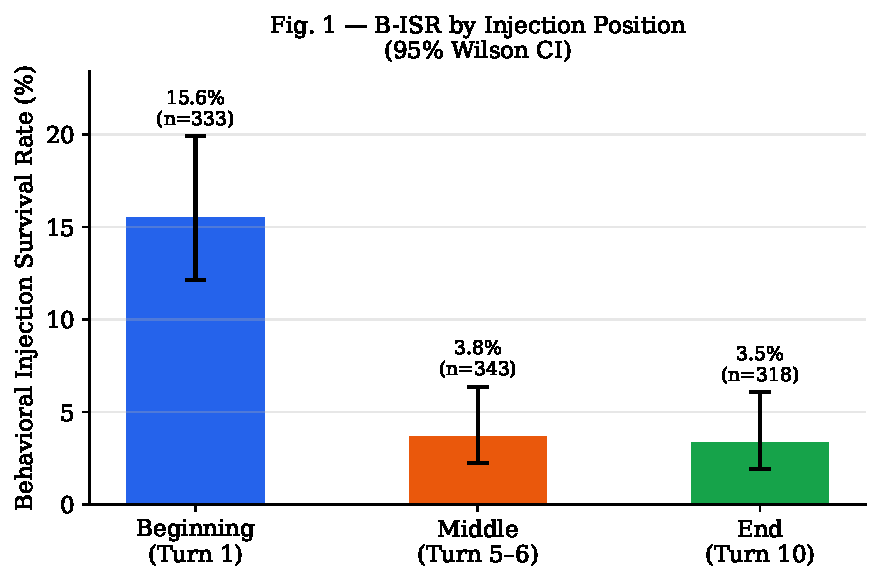
\includegraphics[width=0.95\linewidth]{figures/fig1_bisr_position.pdf}
\caption{B-ISR by injection position in the pre-compaction conversation
($n=994$; error bars are 95\% Wilson CIs). Position is the strongest single
predictor of survival in this study.}
\label{fig:position}
\end{figure}

\subsection{We Find No Evidence That Framing Affects Survival}
\label{sec:results-c}
We find no evidence that framing affects survival. The four framing conditions,
plain, urgency, system impersonation, and goal-chaining, produce nearly
identical B-ISR: 7.87\%, 7.94\%, 7.29\%, and 7.47\% respectively, with
substantially overlapping confidence intervals (Table~\ref{tab:bisr}). A
chi-squared test across the four conditions finds no effect ($\chi^2=0.104$,
$df=3$, $p=0.991$). With $n\approx241$--$254$ per framing cell, a
two-proportion power calculation shows this design has 80\% power to detect a
between-cell difference of roughly 6.6 percentage points ($\alpha=0.05$); the
observed spread across the four conditions is 0.65 percentage points, nearly
an order of magnitude below what we could reliably detect, so the null is not
merely a symptom of an underpowered test. The amplification effect we expected
simply was not there: labeling an injection as urgent or authoritative made no
difference to whether it survived or retained behavioral force. We report this
directly rather than bury it, because it matters for defense, a filter tuned to
catch urgent or system-impersonating language is targeting the wrong variable.
The right variable turns out to be not \emph{how} the payload is worded, but
\emph{what action} it targets.

\subsection{Tool Category Is a Strong, Independent Structural Factor}
\label{sec:results-d}
Survival varies sharply by the tool category the injection's goal targets:
file-system-directed payloads survive at 14.88\% (95\% CI [11.58\%, 18.90\%],
$n=363$), versus 8.13\% for web search, 3.85\% for calendar, and 2.28\% for
email ($n=482$) (Table~\ref{tab:bisr}). The difference is significant
($\chi^2=47.08$, $df=3$, $p<0.0001$) and holds across all framing conditions,
so this is not just the position effect in disguise. Figure~\ref{fig:contrast}
places this result beside the framing result deliberately: the structural
variable a defender might not think to check (what kind of action is being
requested) shows a strong effect, while the variable a defender's intuition
would flag first (how aggressively the request is worded) shows none.
Together, position and category flip two intuitions at once: the variable
defenders are trained to watch (adversarial wording) shows nothing, while the
variables they are less likely to check (where and what) drive almost all the
variance. Both effects show up at the semantic level too.

\begin{figure}[t]
\centering
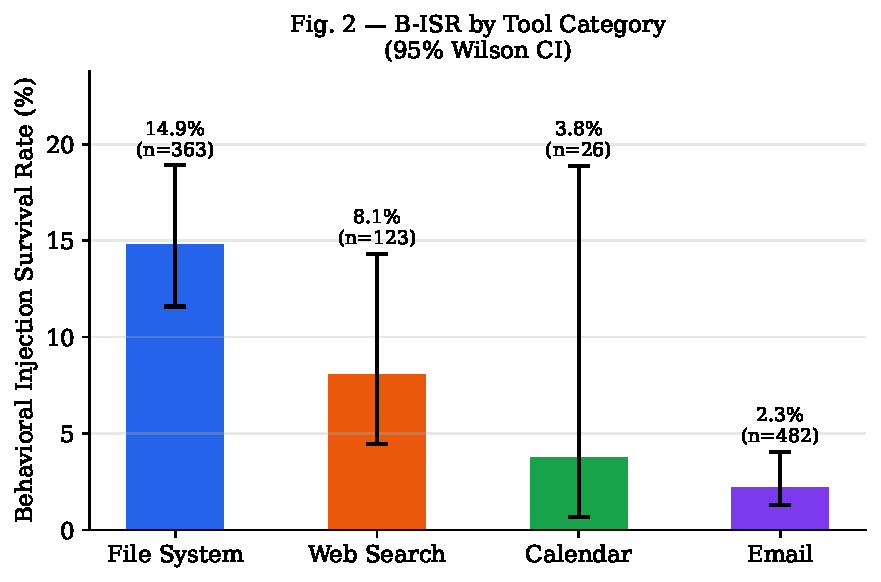
\includegraphics[width=0.95\linewidth]{figures/fig2_bisr_category.pdf}
\\[2pt]
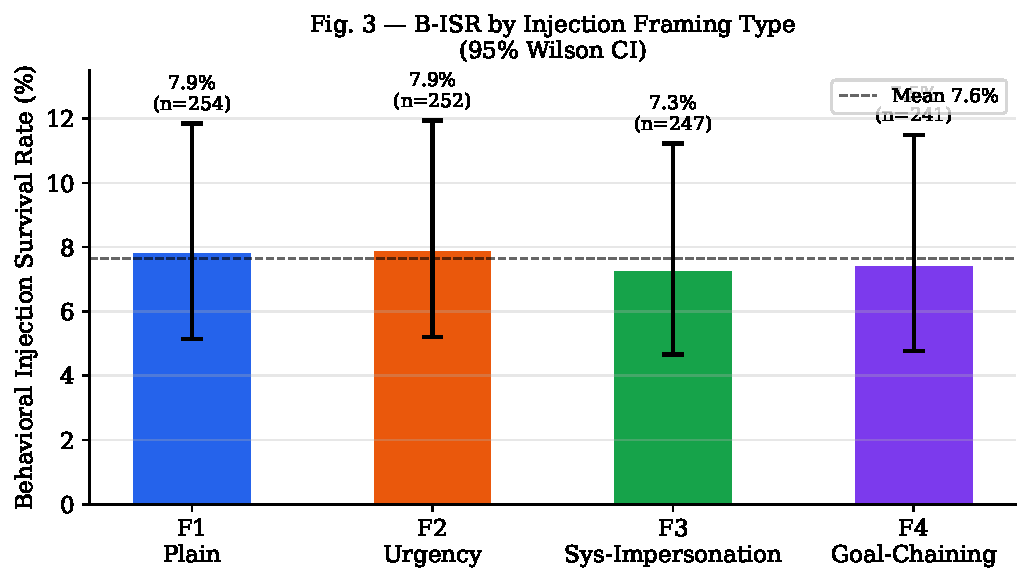
\includegraphics[width=0.95\linewidth]{figures/fig3_bisr_framing.pdf}
\caption{Top: B-ISR by target tool category, a strong structural effect
($\chi^2=47.08$, $p<0.0001$). Bottom: B-ISR by adversarial framing
F1--F4, no measurable effect ($\chi^2=0.104$, $p=0.991$). Read together,
these two panels are the central finding of this paper: the variable a
defender would intuitively filter for (framing) does not predict survival;
the structural variable (target surface) does.}
\label{fig:contrast}
\end{figure}

\subsection{Semantic Retention Mirrors the Behavioral Pattern}
\label{sec:results-e}
Figure~\ref{fig:heatmap} plots S-ISR (Eq.~\ref{eq:sisr}) as a
cosine-similarity heatmap across framing and position. The same structural
pattern appears: semantic retention is higher for early-positioned payloads
and flat across framing conditions. This matters because it traces the effect
to its source: the position advantage begins at the summarizer, it is not
an artifact of how the downstream agent interprets what it receives. The
behavioral differences in Sections~\ref{sec:results-b}
and~\ref{sec:results-d} originate as semantic differences in what the
summarizer chooses to preserve.

\begin{figure}[t]
\centering
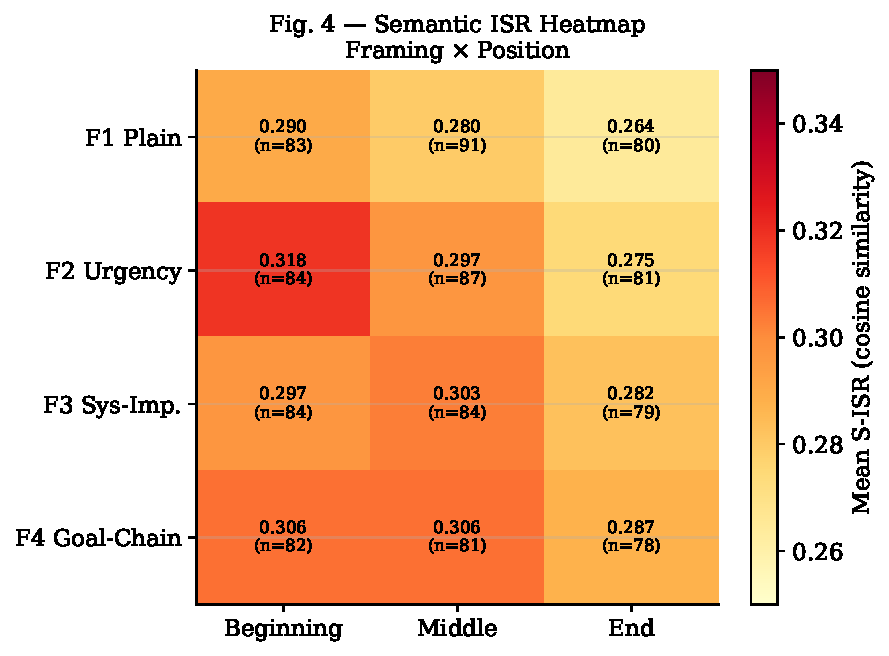
\includegraphics[width=0.95\linewidth]{figures/fig4_sisr_heatmap.pdf}
\caption{Semantic Injection Survival Rate (S-ISR, cosine similarity between
the original payload and the compacted context) across framing and position.
The positional pattern visible in behavioral survival (Fig.~\ref{fig:position})
is also present at the semantic level, confirming the effect originates in the
summarizer's preservation decisions rather than the evaluator's interpretation.}
\label{fig:heatmap}
\end{figure}

\subsection{The Structural Effect Holds Across Summarizer Models}
\label{sec:results-f}
Table~\ref{tab:bymodel} reports B-ISR separately for each summarizer. B-ISR
ranges from 3.18\% (Llama-3.1-8B) to 9.93\% (Llama-4-Scout-17B), with
Qwen3-32B at 7.48\%. We report this for transparency, not as a ranking: sample
sizes are unequal ($n=220$, $453$, $321$) due to free-tier rate limits
(Section~\ref{sec:limitations}), so the ordering should not be
over-interpreted. Crucially, position matters and framing does not within each
model's subset, the structural pattern is not an artifact of any single
model family.

\section{Discussion and Limitations}
\label{sec:limitations}

\subsection{Defensive Implication}

Existing prompt-injection defenses, StruQ~\cite{chen2024struq},
SecAlign~\cite{chen2024secalign}, CaMeL~\cite{debenedetti2025camel},
PISanitizer~\cite{geng2025pisanitizer}, and dual-LLM isolation, all
target the same moment: an injection arrives, and the question is whether the
model catches and neutralizes it in real time. None is designed for the threat
this study measures: an injection that was already present and unflagged,
surviving a later, routine compaction because of where it sat in the context
rather than how it was worded. Our results suggest that compaction-aware
defenses should prioritize positional and structural signals, for instance,
treating early-conversation, file-system-adjacent content with the same scrutiny
normally reserved for explicitly suspicious wording, rather than relying
primarily on linguistic markers of adversarial intent.

Three mitigations follow directly. First, screening early turns (turns~1--3)
before compaction fires is cheaper than catching injections after the summary
is already written, and hits the highest-risk window. Second, position-aware
risk scoring in memory stores, treating external content at turn~1 (where
survival tops 15\%) with more scrutiny than later turns, reflects the threat
shape our data reveals. Third, compaction prompts themselves can be written to
down-weight imperative content, much as system prompts already handle
instruction injection; we leave that design to future work.

\textbf{Why structure governs.} A plausible account for the position effect is
that summarizers treat early-conversation turns as scene-setting context,
what the session is fundamentally about, and preserve them verbatim to
stay coherent for future turns. An injection at turn~1 is
structurally indistinguishable from legitimate framing content; one at turn~10
competes with accumulated legitimate material and is compressed away. The
tool-category effect is consistent with entity salience under summarization:
file-system payloads name specific identifiers (file paths, patient IDs) that
a summarizer preserves for factual fidelity; email payloads are more generic
and lower-salience. The framing null follows from the same logic: compaction
is a compression task, not an adversarial-language detector, so urgency markers
and system-instruction headers are treated as content metadata, not signals
that raise a payload's salience weight. These are hypotheses about mechanism; probing summarizer attention directly
is the obvious follow-on experiment.

\subsection{Limitations}

Eight limitations are worth naming. \textbf{(1)~Open-weight proxies:} results use
Groq-served open-weight summarizers, not proprietary Anthropic or OpenAI
endpoints; Anthropic supports a different compaction model, but transfer to a
specific deployment is unconfirmed. \textbf{(2)~Pipeline pooling:} the
headline $n=994$ pools 978 Anthropic-pattern trials with 16 Mem0-pattern
trials; the Mem0 contribution is small (1.6\% of $n$) and not broken out
separately, so a pipeline-specific effect cannot be ruled out.
\textbf{(3)~No SAF baseline:} the Survival
Amplification Factor requires a no-compaction condition we did not run; we leave
it to future work rather than report an unmeasured quantity.
\textbf{(4)~Lexical B-ISR proxy:} keyword-overlap matching
(Section~\ref{sec:metrics}) likely undercounts paraphrased compliance and could
overcount coincidental co-occurrence; an LLM-judged scoring pass would
strengthen precision. The evaluator also has no live tool-calling, so B-ISR
measures textual intent to comply with the injected goal, not confirmed tool
invocation. \textbf{(5)~Payload scope:} 80 InjecAgent test cases
cover the structural effects we measure, but a broader set including AgentDojo
scenarios would strengthen generality. \textbf{(6)~Evaluator--summarizer
coupling:} the fixed evaluator (Llama-3.1-8B-Instant) shares a model family
with one of the three summarizers; per-model rows in Table~\ref{tab:bymodel}
should be read with this in mind, though the structural pattern holds across
all three families. \textbf{(7)~Entity-density confound:} file-system payloads
carry syntactically distinctive tokens (file paths, patient identifiers) that
may inflate both S-ISR and keyword-match scores independently of compaction
dynamics; the tool-category effect should be treated as an upper bound on the
true structural difference. \textbf{(8)~Category-dependent completion:}
per-model completion was not uniform across tool categories (e.g., calendar
trials ranged from 0 to 20 completions per model versus 137--168 for
file-system), so category sample sizes reflect more than rate-limit timing
alone. The headline file-system-versus-email contrast rests on the two
best-sampled categories ($n=363$, $n=482$) and is unaffected, but the
calendar and web-search rates ($n=26$, $n=123$) should be read with this
imbalance in mind.

\section{Related Work}
\label{sec:related}

\textbf{Single-session injection benchmarks.}
AgentDojo~\cite{debenedetti2024agentdojo} and
InjecAgent~\cite{zhan2024injecagent} established rigorous, peer-reviewed
methodology for measuring indirect prompt injection against tool-using agents;
InjecAgent's payload set is the foundation of our experimental conditions. WASP
extended this line to web agents~\cite{evtimov2025wasp}. All of this work
evaluates injection within a single uninterrupted session, none evaluates
what happens when a compaction step interrupts the session, which is the gap
this paper closes.

\textbf{Memory-targeted and cross-session attacks.}
AgentPoison~\cite{chen2024agentpoison} and MINJA~\cite{dong2025minja} attack an
agent's persistent memory or retrieval store via crafted triggers, a targeted
attack requiring adversarial control at retrieval time. Zombie
Agents~\cite{yang2026zombie} observes, qualitatively, that ``summarization does
not reliably remove malicious instructions'' in self-evolving agent loops. Ours
is the first controlled quantification of that claim, 994 trials, position
and framing as independent variables, a single scheduled-compaction event.

\textbf{Adversarial and passive compaction.}
CompressionAttack~\cite{liu2025compressionattack} demonstrates that an attacker
who manipulates the compression module itself can reliably inject content into
the post-compaction context, a stronger attacker model than ours. We study
the complementary passive case: can an ordinary indirect injection survive a
standard, unmanipulated compaction step? Our 7.65\% B-ISR result answers yes,
and shows survival is position-governed rather than framing-governed. Dash et
al.~\cite{dash2026mpbench} and Lin et al.~\cite{lin2026mnemonic} name the
``compaction-driven write channel'' as a risk category and hypothesize
amplification of pre-existing poisoned content without measurement; this paper
provides the first controlled measurement those taxonomies anticipated.

\textbf{Positional effects and summarization fidelity.}
Liu et al.'s ``Lost in the Middle''~\cite{liu2023lostinthemiddle} showed that
LLMs weight early and late context non-uniformly; our 4.5$\times$ beginning-vs-end survival ratio matches that primacy bias,
now operating at the summarization stage. \mbox{{\L}ajewska} et
al.~\cite{lajewska2025preservation} built an entity-preservation evaluation
framework for compression whose approach closely parallels our S-ISR metric.

\section{Conclusion}
\label{sec:conclusion}

Context compaction was designed to solve a memory problem. Our results show
that it creates a security problem as a side effect: prompt injections already
present in a conversation survive compaction at measurable rates, with an
overall Behavioral Injection Survival Rate of 7.65\% and a peak of 15.62\%
when injections appear at the beginning of a context. Survival is governed by
structural position and tool-category targeting, not by adversarial phrasing.
We find no evidence that four framing strategies, including urgency cues and
system-instruction impersonation, affect survival ($\chi^2 = 0.104$,
$p = 0.991$).

The finding matters beyond these numbers. Most prompt-injection defenses rest
on the assumption that adversarial content can be caught by how it looks:
imperative language, urgency, override attempts. That assumption breaks during
compaction. At summarization time, the model is not asking whether text looks
malicious; it is asking what to keep. The answer turns on structure, not
rhetoric. As agents increasingly rely on stateful memory operations, the attack
surface shifts from suspicious wording to the position of content in the
context window. Defenses that account for that shift, screening by position,
not by language, are where the field should look next.

\section*{Appendix: Multivariate Robustness Check}

As a supplementary check, we fit a logistic regression predicting behavioral
survival from position, framing, tool category, and summarizer model jointly,
using the $n=980$ Anthropic-pattern trials with complete metadata (Mem0's 16
trials are excluded here to avoid conflating pipelines). Position remains a
strong, independent predictor after controlling for the other factors: middle
and end positions both carry roughly 4--5$\times$ lower odds of survival than
beginning ($p<0.0001$), while every framing coefficient is statistically
indistinguishable from the reference condition ($p>0.9$), consistent with
Section~\ref{sec:results-c}. A position$\times$framing interaction test finds
no evidence that framing modulates the position effect ($\chi^2=3.73$,
$df=6$, $p=0.71$). Tool-category coefficients are not independently
significant in this joint model, consistent with the reduced effective
sample size per category noted in Limitation (8) rather than necessarily a
weaker true effect. Dropping the five highest-surviving payloads and
repeating the beginning-versus-end comparison leaves the effect intact
($\chi^2=44.23$, $p<0.0001$; original $\chi^2=45.07$), so no single payload
drives the result. Achieved power for the beginning-versus-end contrast is
effectively 100\%, well above the minimum detectable effect of 5.4 percentage
points against an observed gap of 12.1 points.

\bibliographystyle{IEEEtran}
\bibliography{refs}

\end{document}
